\documentclass[a4paper,11pt]{article}
%\usepackage[T1]{fontenc}

%\setlength{\textwidth}{20cm}
%\setlength{\marginparwidth}{0cm}
%\setlength{\voffset}{0cm}
\usepackage[utf8]{inputenc}
\usepackage[francais]{babel}
\usepackage{amsmath}
\usepackage{graphicx}
\usepackage{slashbox}

%\special{papersize=210mm,297mm}

\title{{\Huge Electronique numérique}\\Automates (2)\\CORRECTIONS}
\date{}

\begin{document}
\maketitle
{\it Tous les exercices ne seront pas forcément résolus en TE.}

\section{Problème de modélisation séquentielle}
Le circuit suivant doit commander un passage à niveau.

\begin{figure}[!h]
\begin{center}
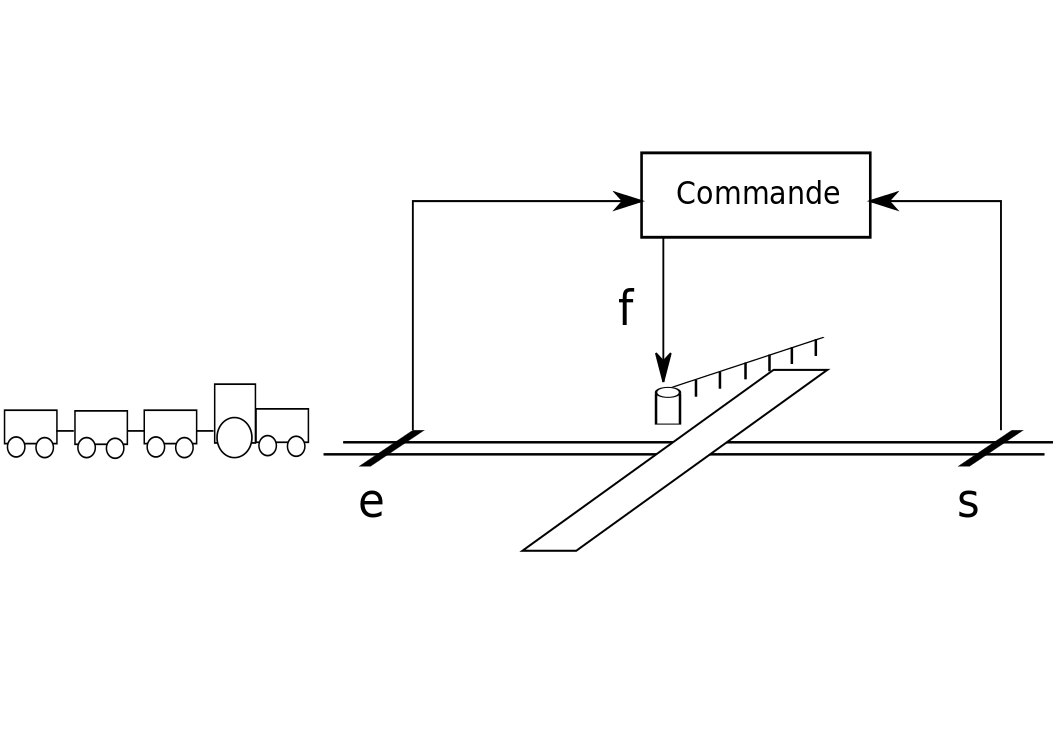
\includegraphics[scale=0.3]{./train.png}
\end{center}
\end{figure}

Deux capteurs $e$ (entrée) et $s$ (sortie) signalent l'entrée et la sortie d'un train ; les signaux $e$ et $s$ durent exactement 1 cycle pour le passage d'un train; il peut y avoir au maximum 2 trains entre les points $e$ et $s$ ; un train peut entrer alors que simultanément un autre sort ; le passage à niveau doit être fermé s'il y a au moins un train entre $e$ et $s$.

\subsection*{Questions}

\begin{enumerate}
\item Donner un diagramme d'état (``à bulles'') du circuit de commande.
\item Réaliser ce circuit à l'aide de bascules D.
\end{enumerate}

{\bf solution (partielle)}

\begin{figure}[!h]
\begin{center}
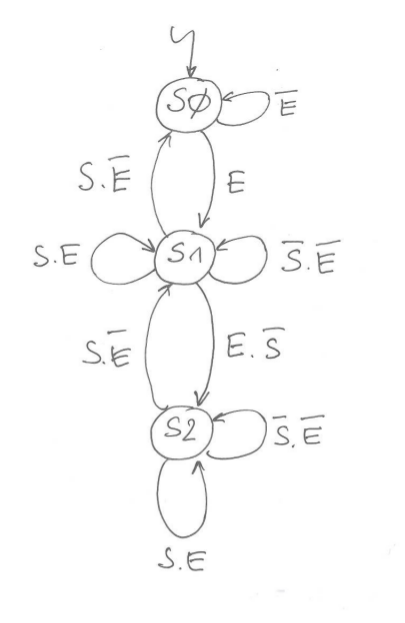
\includegraphics[scale=0.4]{./sol5-1.png}
\end{center}
\end{figure}

Note : ce sujet simple prête toutefois à des interrogations tout à fait légitimes pour l'ingénieur : dans le dernier état, que se passe-t'il si le signal d'entrée s'active alors que S ne s'active pas ? La spécification du système dit ``{ \it  il peut y avoir au maximum 2 trains entre les points $e$ et $s$}'' , mais est-ce à l'automate de s'en assurer ou est-ce une hypothèse d'entrée parfaitement vérifée par l'environnement ? Il y a là une ambiguité qui devrait être discutée. L'ingénieur responsable peut aussi proposer une solution : la plus raisonnable semble être de rajouter un état d'erreur vers lequel transiter. Dans ce cas, une fois cet état atteint, il faudrait une autre entrée (reset) pour sortir l'automate de cet état...Mais cela peut engendrer un ensemble de conséquences sur le réseau amont et aval...Un tel {\it système électronique} est bel et bien plongé dans un environnement complexe : le ``Système''.

\newpage
\section{Problème du dé électronique}
On doit réaliser une boîte équipée d'un bouton poussoir, de 7 diodes lumineuses (LEDs) d'un circuit logique (à définir) et d'une pile. Ce dispositif doit simuler un dé, lancé aléatoirement : il affiche entre 1 et 6.\\

\begin{figure}[!h]
\begin{center}
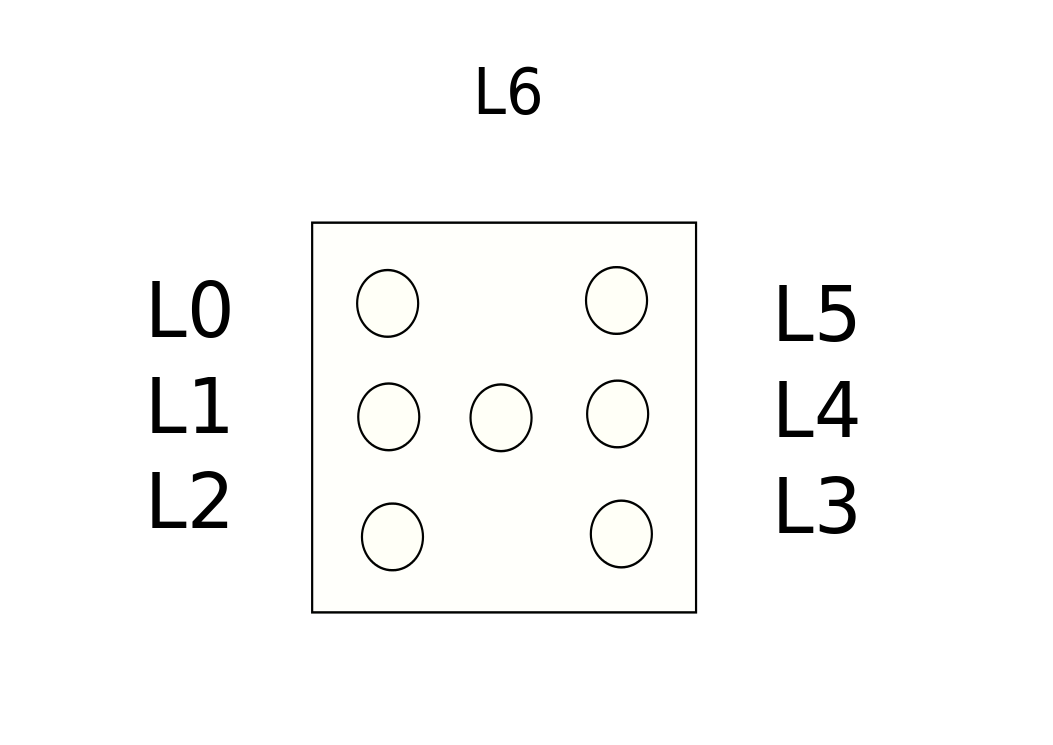
\includegraphics[scale=0.2]{./de-1.png}
\end{center}
\end{figure}


Chaque fois que l'utilisateur appuie sur le bouton-poussoir toutes les leds s'allument puis, dès que l'opérateur relâche le bouton, les LEDs se fixent à l'une des configurations ci-dessous.\\

A l'appui sur le bouton poussoir toutes les configurations sont affichées en séquence à la cadence d'une horloge rapide. L'utilisateur ne peut pas distinguer les combinaisons, du fait de la persistence rétinienne. Seule une illumination moyenne lui apparait.

\subsection*{Question}
\begin{itemize}
\item Réaliser ce système, de manière à ce que la fonction de sortie de l'automate soit l'identité. Pour cela choisir un encodage des états approprié.
\item Dessiner un schéma-blocs composé de 2 blocs : la logique d'état suivant et les bascules D (registres).
\item Choisir un autre encodage (par exemple one-hot) et réaliser à nouveau le circuit.
\end{itemize}


\section{Du diagramme à bulles au circuit. Exemple de l'arbitre à priorité tournante (round-robin)}
On rappelle que le diagramme à bulle est une représentation, qui se veut intuitive, du comportement séquentiel d'un automate d'états finis (FSM) : chaque état est représenté par un cercle
(bulle) duquel peuvent partir différentes transitions (ou arcs) vers d'autres états possibles. Les transitions sont étiquetées par la condition booléenne amenant à l'état suivant.\\

On désire réaliser un circuit d'arbitrage entre deux clients susceptibles d'utiliser une ressource qui n'admet qu'un seul occupant à la fois (par exemple deux enfants qui veulent jouer au vélo,
et il n'y a qu'un vélo. Le cas se présente également dans les ordinateurs, où différents périphériques peuvent vouloir accéder à un ensemble de fils --bus central-- en même temps).
Le but du circuit est d'accorder correctement la ressource à un seul client à la fois.\\

Les clients manifestent respectivement sur $e_1$ et $e_2$ leurs désirs d'utiliser la ressource : $e_i=1$ si le client $i$ désire la ressource, $e_i=0$ s'il ne la désire pas.\\

\begin{figure}[!h]
\begin{center}
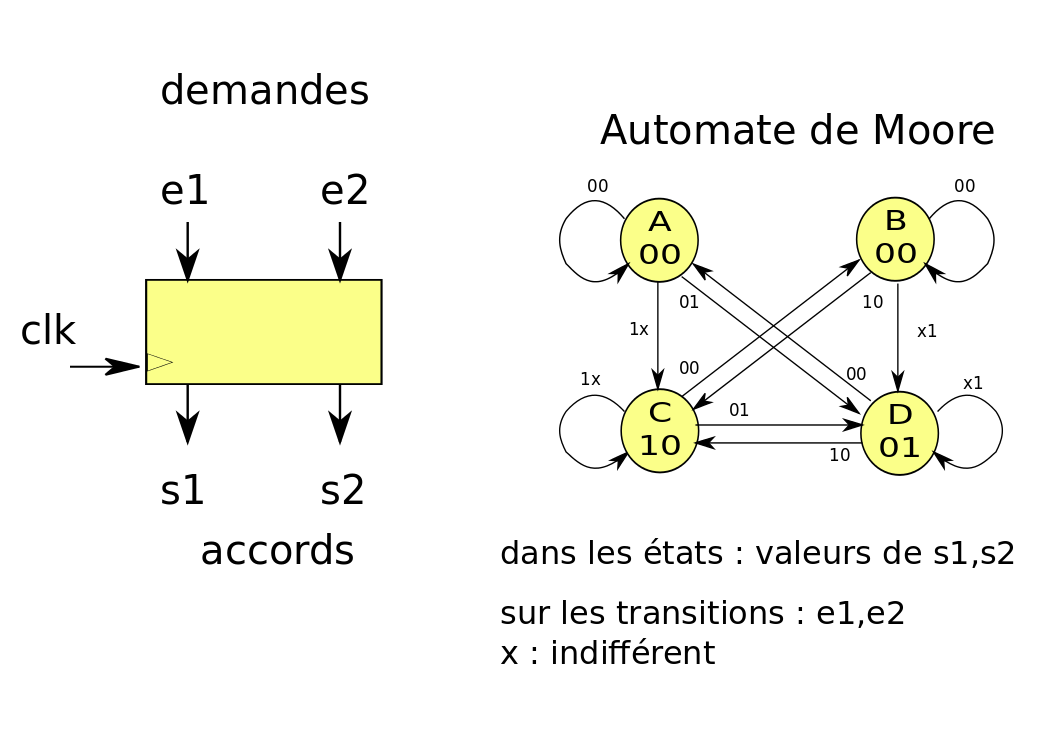
\includegraphics[scale=0.3]{./arbitre.png}
\end{center}
\end{figure}

Le circuit génère sur $s_1$ et $s_2$ l'attribution de la ressource à chaque client : $s_i=1$ si la ressource est attribuée au client $i$, $s_i=0$ sinon.\\

Lorsque la ressource est attribuée à un client, elle le demeure tant que le client la désire.\\

Lorsque la ressource est libre, elle est attribuée au premier qui la demande ; en cas de demandes simultanées, elle est attribuée selon une certaine priorité, mais pour éviter les injustices, la priorité entre les clients change à chaque attribution : le client qui obtient la ressource devient le moins prioriatire.\\

L'analyse du problème conduit à l'automate suivant : il y a quatre états, deux états A et B dans lesquels la ressource est libre, et deux états C et D dans lesquels la ressource est occupée.

\subsection*{Questions}
\begin{enumerate}
\item Proposer un encodage des états tel que chaque état soit codé sur 2 bits
\item Etablir la fonction de transition du système sous forme de table de vérité. Simplifier.
\item Etablir la fonction de sortie du système. Simplifier.
\item Dessiner le circuit correspondant. Combien de portes faut-il ?
\end{enumerate}

\newpage
{\bf solutions}

%On propose l'encodage des états a priori le plus intuitif : $A\rightarrow 00$, $B \rightarrow 01$, $C \rightarrow 10$, $D \rightarrow 11$ etc...
Cet encodage nous indique qu'il faut 2 bascules D pour stocker l'état du système. Nommons par exemple ces deux bascules $Q_1$ et $Q_0$.

\begin{figure}
\begin{center}

      \begin{tabular}{|c||c|c|cc|}
          \hline
          Etat  & Encodage entier & Encodage binaire & $Q_1$ & $Q_0$ \\ \hline \hline
          A     & 0 & 00 & 0 & 0 \\ \hline
          B     & 1 & 01 & 0 & 1 \\ \hline
          C     & 2 & 10 & 1 & 0 \\ \hline
          D     & 3 & 11 & 1 & 1 \\ \hline
      \end{tabular}
\end{center}
\end{figure}

Ecrivons la table qui décrit l'évolution des entrées des bascules en fonction des entrées et de l'état courant. Dans le tableau, on a rappelé les états symboliques.

\begin{figure}
\begin{center}
      \begin{tabular}{|c|c|c|c|c||c|c|c|}
          \hline
          \multicolumn{3}{|c|}{Etat courant} & \multicolumn{2}{c||}{Entrées} & \multicolumn{3}{c|}{Etat futur} \\ \hline
          symbole  & $Q_1$ & $Q_0$ & $e_1$ & $e_2$ & $D_1$ & $D_0$ & symbole  \\ \hline \hline
          A & 0 & 0 & 0 & 0 & 0 & 0  & A \\ \hline
          A & 0 & 0 & 0 & 1 & 1 & 1 & D  \\ \hline
          A & 0 & 0 & 1 & 0 & 1 & 0 & C\\ \hline
          A & 0 & 0 & 1 & 1 & 1 & 0 & C\\ \hline \hline
          B & 0 & 1 & 0 & 0 & 0 & 1  & B\\ \hline
          B & 0 & 1 & 0 & 1 & 1 & 1  & D\\ \hline
          B & 0 & 1 & 1 & 0 & 1 & 0  & C\\ \hline
          B & 0 & 1 & 1 & 1 & 1 & 1  & D\\ \hline \hline
          C & 1 & 0 & 0 & 0 & 0 & 1  & B\\ \hline
          C & 1 & 0 & 0 & 1 & 1 & 1  & D\\ \hline
          C & 1 & 0 & 1 & 0 & 1 & 0  & C\\ \hline
          C & 1 & 0 & 1 & 1 & 1 & 0  & C\\ \hline \hline
          D & 1 & 1 & 0 & 0 & 0 & 0  & A\\ \hline
          D & 1 & 1 & 0 & 1 & 1 & 1  & D\\ \hline
          D & 1 & 1 & 1 & 0 & 1 & 0  & C\\ \hline
          D & 1 & 1 & 1 & 1 & 1 & 1  & D\\ \hline
      \end{tabular}
\end{center}
\end{figure}
partir de ce tableau, on cherche les équations de $D_1$ et $D_0$. $D_1$ se trouve facilement, par une observation attentive du tableau : on peut voir une factorisation aisée :
$$D_1=e_1+e_2$$
Pour $D_0$, passons par un tableau de Karnaugh.

\begin{figure}
   \begin{center}
      \begin{tabular}{|c|c|c|c|c|}
        \hline
                \backslashbox{$Q_1.Q_0$}{$e_1.e_2$}  & 00 & 01 & 11 & 10 \\ \hline
                                                 00 &  ~ &  1 &  ~ & ~ \\
                                                 00 &  1 &  1 &  1 & ~ \\
                                                 01 &  ~ &  1 &  1 & ~ \\
                                                 11 &  1 &  1 &  ~ & ~ \\ \hline
      \end{tabular}
   \end{center}
\end{figure}
Les regroupements amènent à :
$$D_0=\overline{e_1}.e_2+e_2.Q_0+\overline{e_1}.\overline{Q_1}.Q_0+Q_1.\overline{Q_0}.\overline{e_1}$$

Calculons les sorties, de la même manière. On trouve : $S_1=Q_1.\overline{Q_0}$ et $S_2=Q_1.Q_0$

On peut désormais dessiner le circuit complet :

\begin{figure}[!h]
\begin{center}
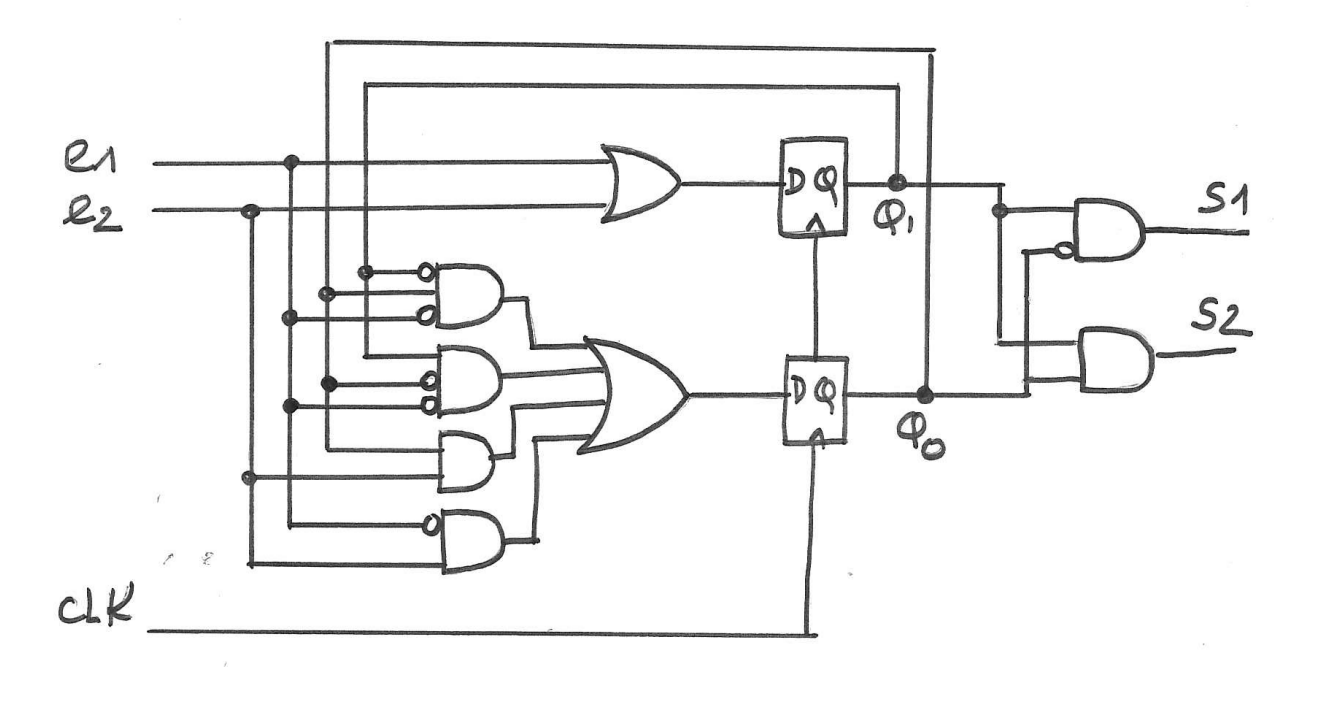
\includegraphics[scale=0.3]{./circuit-4.png}
\end{center}
\end{figure}

\end{document}
